\documentclass[12pt]{article}

\usepackage[utf8]{inputenc}
\usepackage[T1]{fontenc}
\usepackage[english]{babel}
\usepackage{amssymb}
\usepackage[export]{adjustbox} % allows to use extra argument in \includegraphics{imagefile}, e.g.: \includegraphics{imagefile, center}
\usepackage{amsmath}
\usepackage[hidelinks]{hyperref}



\title{Report: Assignment 1: \\Big Data Analytics Programming}
\author{Andreas Hinderyckx}
\date{December 2021} 

\usepackage{graphicx}
\usepackage{xcolor}
\usepackage{caption}

\begin{document}

\newcommand{\todo}{\fbox{\textbf{\textcolor{red}{TODO}}} }
\newcommand{\sctf}[1]{10\mathrm{e}{-#1}}
\maketitle

\newpage

%\section{Bugs}\todo
\section{Learning Curves}
All the learning curves discussed in this section are plotted with the default parameters ($\text{PERIOD } = 10^5, \eta = 10^{-9}, n_{min} = 200, \tau = 0.05 \text{ and } \delta = 10^{-7}$). The weights of the Perceptron are initialised to zeroes (see section \ref{sec:experiments}).

The learning curves for the Perceptron (PC) and Very Fast Decision Tree (VFDT) run on the \texttt{clean} datasets are shown in figures \ref{fig:pc_clean} and \ref{fig:vfdt_clean} respectively. The accuracy of the PC shows much more volatility whereas the VFDT's accuracy follows a more stable course which, however, only reaches about $77\%$. After around $100.000.000$ examples have been trained with, we can clearly see the change of model used to generate the data in both graphs: both the PC's and VFDT's accuracy take a steep drop. The PC quickly recovers back up to its original state, whereas the VFDT doesn't reach the same accuracy it had before: this could be due to the VFDT being overfit to the previously used model to generate the data, whereas the PC's weights can be changed entirely as needed.	

Tested on the \texttt{noisy} data set, we acquire the learning curves shown in figures \ref{fig:pc_noise} and \ref{fig:vfdt_noise}. Now, the volatility of the PC's accuracy becomes clearly visible: it struggles to learn the model due to the added noise. The VFDT's graph is highly similar to its graph for the \texttt{clean} data, with a reduction of achieved accuracy of $10\%$ and some extra volatility.


\begin{figure}
	\centering
	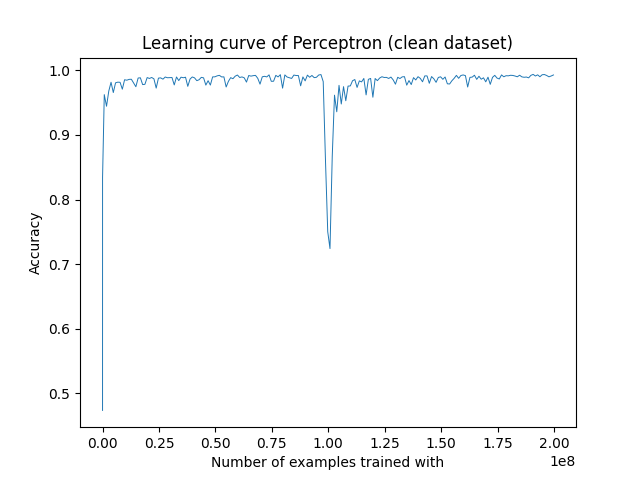
\includegraphics[width=.8\linewidth]{../plots/pc_clean}
	\caption{Learning curve of PC on the \texttt{clean} dataset}
	\label{fig:pc_clean}
\end{figure}
\begin{figure}
	\centering
	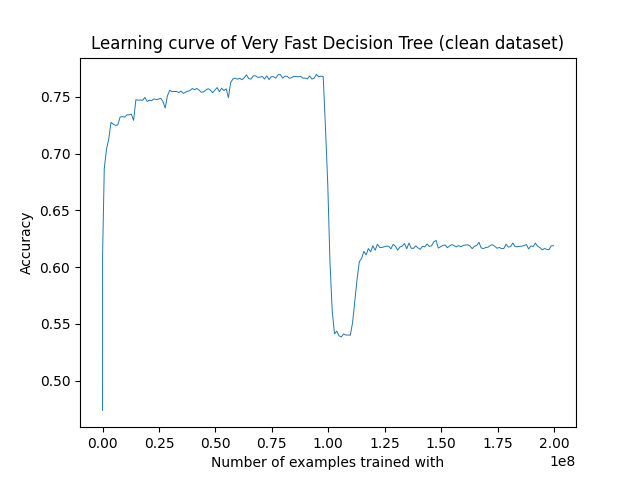
\includegraphics[width=.8\linewidth]{../plots/vfdt_clean}
	\caption{Learning curve of VFDT on the \texttt{clean} dataset}
	\label{fig:vfdt_clean}
\end{figure}
\begin{figure}
	\centering
	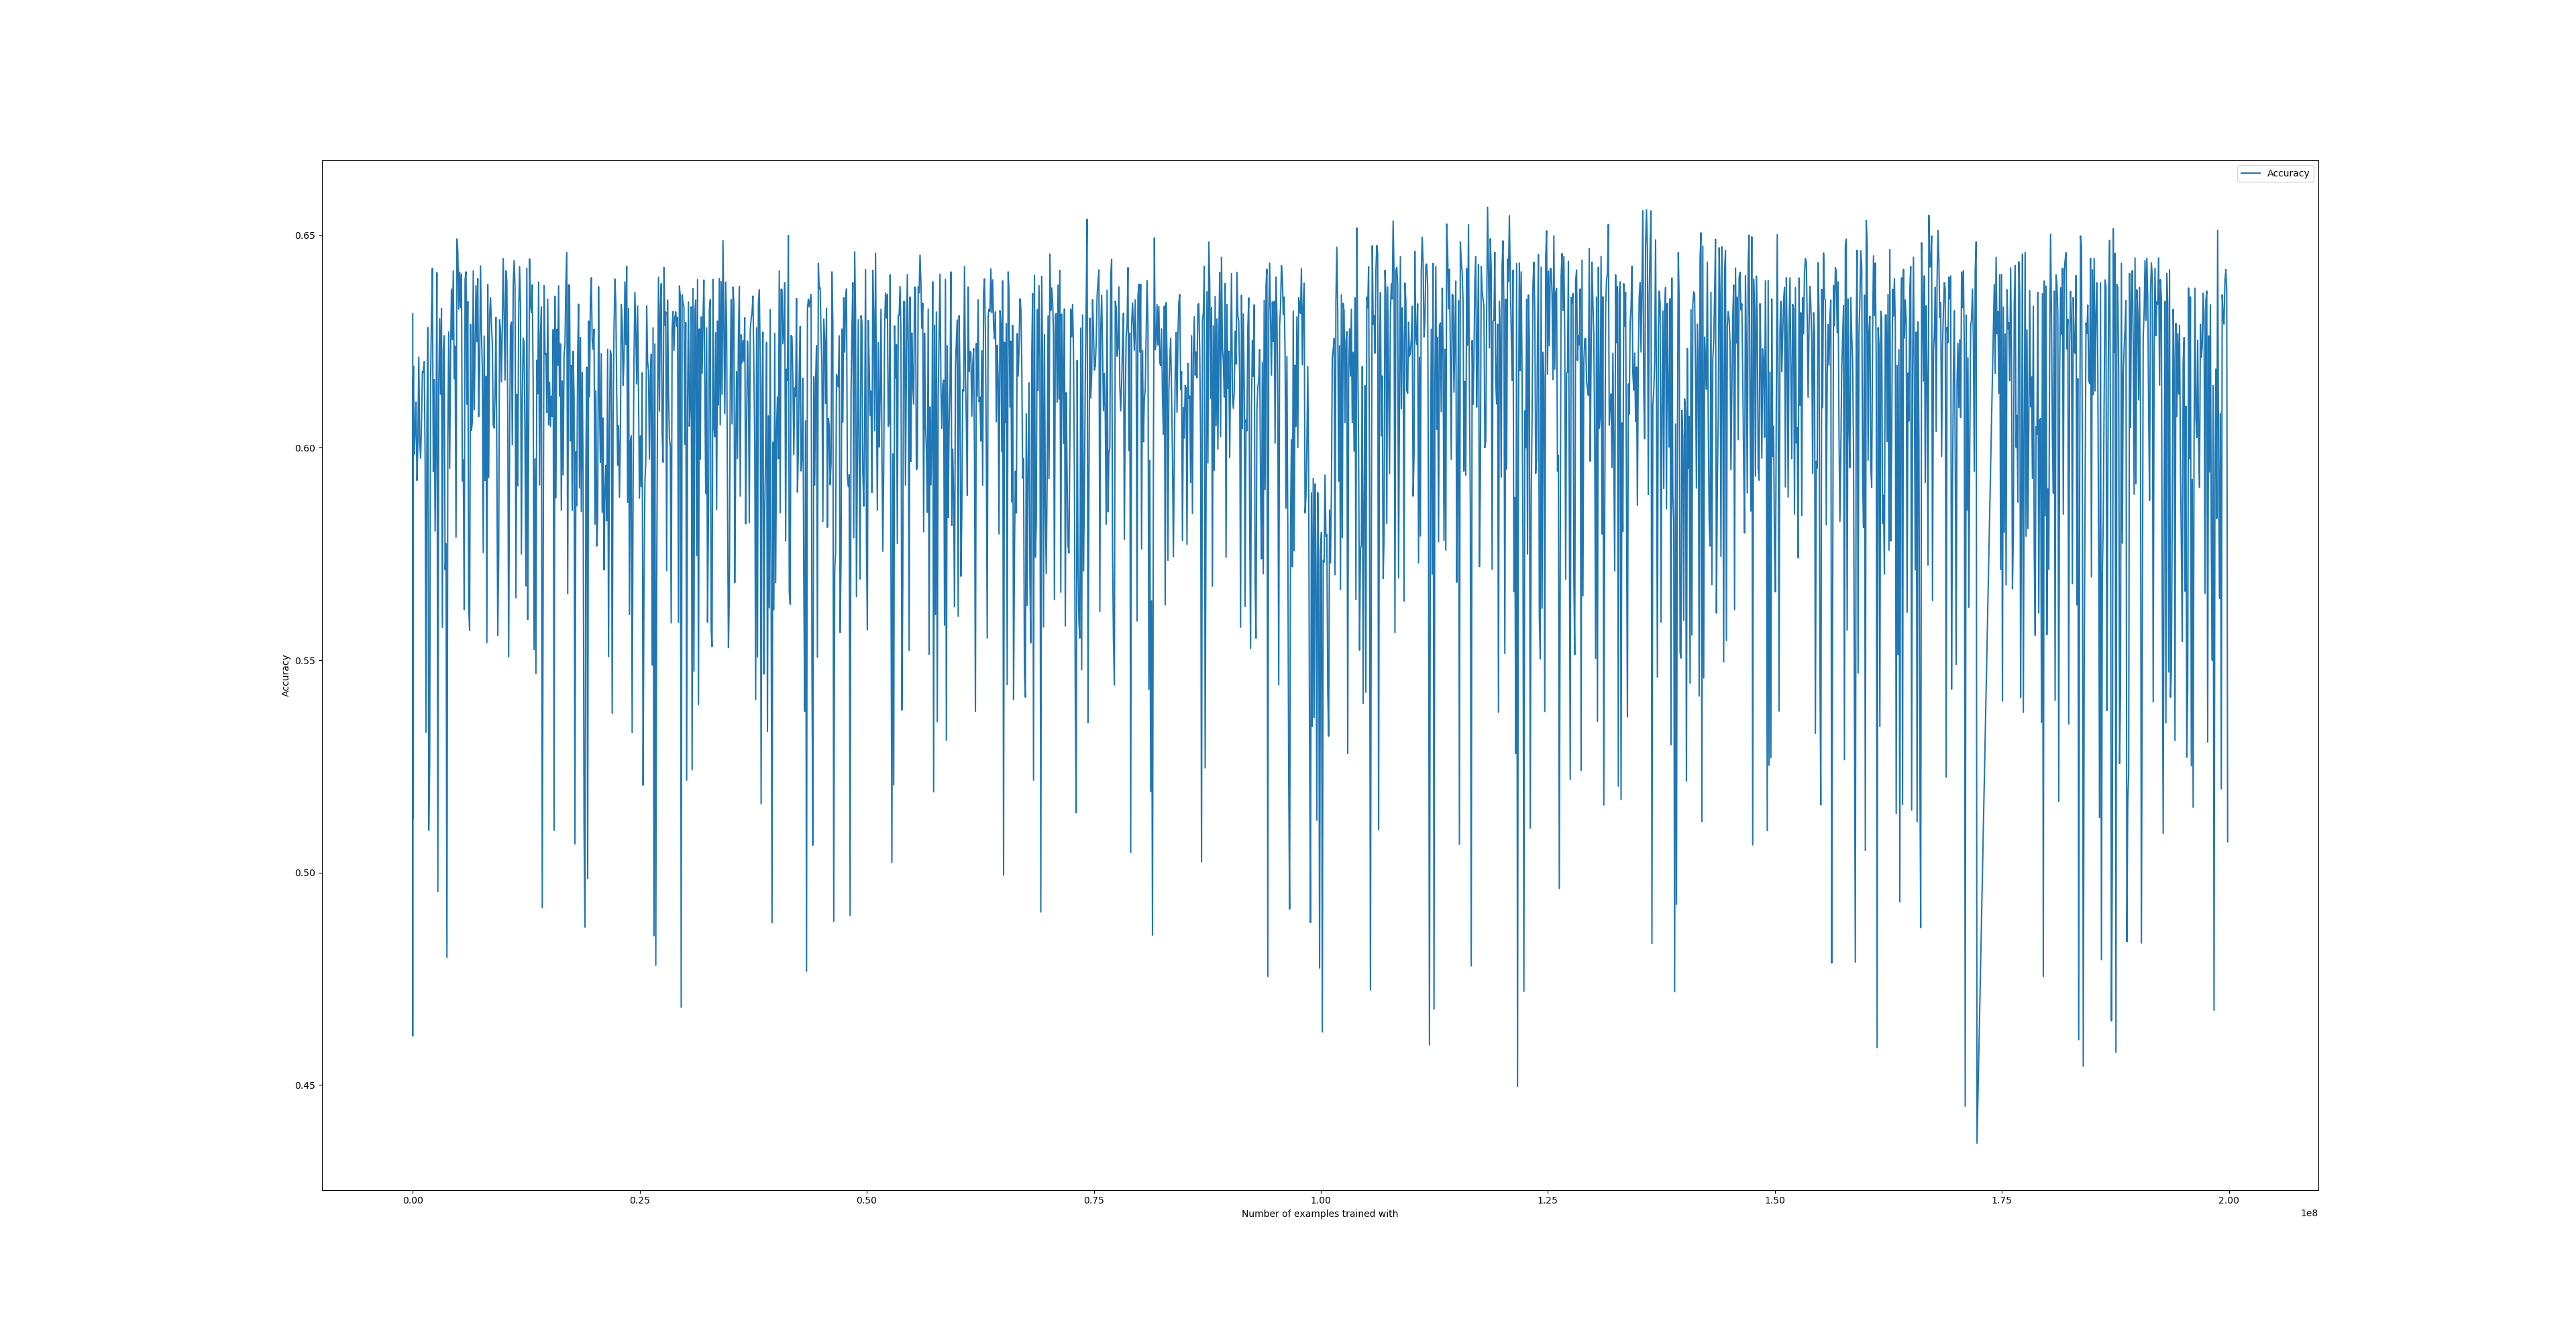
\includegraphics[width=.8\linewidth]{../plots/pc_noise}
	\caption{Learning curve of PC on the \texttt{noisy} dataset}
	\label{fig:pc_noise}
\end{figure}
\begin{figure}
	\centering
	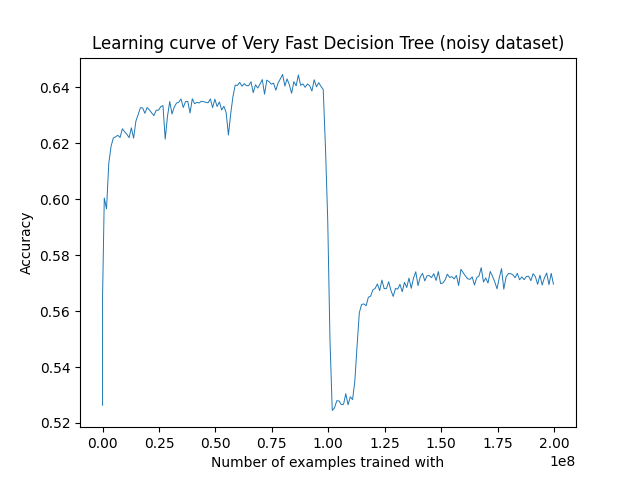
\includegraphics[width=.8\linewidth]{../plots/vfdt_noise}
	\caption{Learning curve of VFDT on the \texttt{noisy} dataset}
	\label{fig:vfdt_noise}
\end{figure}

\section{Experiments}\label{sec:experiments}
To study the effect of different parameters present in the programs, we pose the following questions:
\begin{enumerate}
	\item What's the effect of non-zero initialisation of the weights of the PC?
	\item What's the effect of varying $\eta$ (eta: learning rate) in the PC implementation?
	\item What's the effect of varying $\delta$ (delta) in the VFDT implementation?
	\item What's the effect of varying $\tau$ (tau) in the VFDT implementation?
	\item What's the effect of varying $n_{min}$ (how often split function is recalculated) in the VFDT implementation?
\end{enumerate}

We set up experiments in which we vary the parameters specified in the mentioned questions above and become the following results.

For different values of $\eta$ to take effect on the model, we must initialise the PC's weights to non-zero values\footnote{\url{https://datascience.stackexchange.com/a/27305}}. We initialise the weights with normally distributed values with $\mu = 0 \text{ and } \sigma = 0.001$. The learning curves for the PC with varying values for $\eta$ on the \texttt{clean} data set are shown in figure \ref{fig:pc_etas}. We notice that $\eta$ must be sufficiently large in order for the model to gain accuracy: $\eta = 10^{-9}$ is sufficient to increase accuracy, albeit at a very slow rate due to the small updates. Taking $\eta \geq 10^{-7}$ yields much quicker accuracy gains at the cost of more volatility, and	 doesn't quite reach the same final accuracy as with $\eta = 10^{-9}$, due to the learning rate being too large to make precise adjustments to the weights to try to increase the accuracy further beyond $\sim 97\%$.

For studying the parameters of the VFDT, we use the \texttt{clean} dataset. In figure \ref{fig:vfdt_deltas} we can see that varying $\delta$ affects the speed at which accuracy is gained: in the first part of the learning curve, larger values for $\delta$ lead to faster gains in accuracy. This is what we expect, as increasing delta implies a less strict Hoeffding bound, which will cause the VFDT to make splits quicklier (see fig. \ref{fig:vfdt_delta_zoom}). After the concept drift, $\delta = 10^{-7}$ increases the accuracy the quickliest: this value possibly hits the right middleground between splitting as quick as possible (larger $\delta$) and not overfitting too much too quickly on the data (smaller $\delta$); cfr. figure \ref{fig:vfdt_delta_zoom2}.

From figure \ref{fig:vfdt_taus} we can deduce that smaller values of $\tau$ increase the learning efficiency: this makes sense as the algorithm spends less time on deciding between minor differences in split evaluations and will be able to split sooner on these cases. We also note that for larger values of $\tau$, the experiments didn't finish due to excessive memory usage, as the algorithm will then split more often and thus consumes more memory as $\tau$ increases.

Finally, increasing $n_{min}$ implies the VFDT will re-compute the split evaluation function less frequently, which decreases computation times (as calculating the split evaluation is the most costly part of the algorithm), but should also decrease the rate at which is learned, as eligible splits are only discovered after a delay of at most $n_{min}$ examples. The latter is confirmed by figure \ref{fig:vfdt_nmins}, of which an enlarged view can be seen in figure \ref{fig:vfdt_nmins_zoom}.

\section{Special points about implementation}
In the implementation of the Perceptron I added a variable \texttt{randomiseWeights} to toggle between the weights being either  initialised to all zeroes or to initialise the weights with randomly normally distributed values with $\mu = 0 \text{ and } \sigma = 0.001$, as mentioned above. This was set to true to verify the effect of changing the value of $\eta$. For the default provided value of the learning rate ($\eta = 10^{-7}$), however, the implementation with weights initialised to all zeroes obtained the best results. Therefore, the weights will by default be initialised to all zeroes (i.e. \texttt{randomiseWeights = false}).

In the method \texttt{addChildren} in \texttt{VfdtNode.java}, the \texttt{nijk} counts of the current node that executes \texttt{addChildren} are set to \texttt{null} after the children are added. These counts are no longer needed from this point on and the memory occupied by them can therefore be made available for garbage collection.



\begin{figure}
	
	\centering
	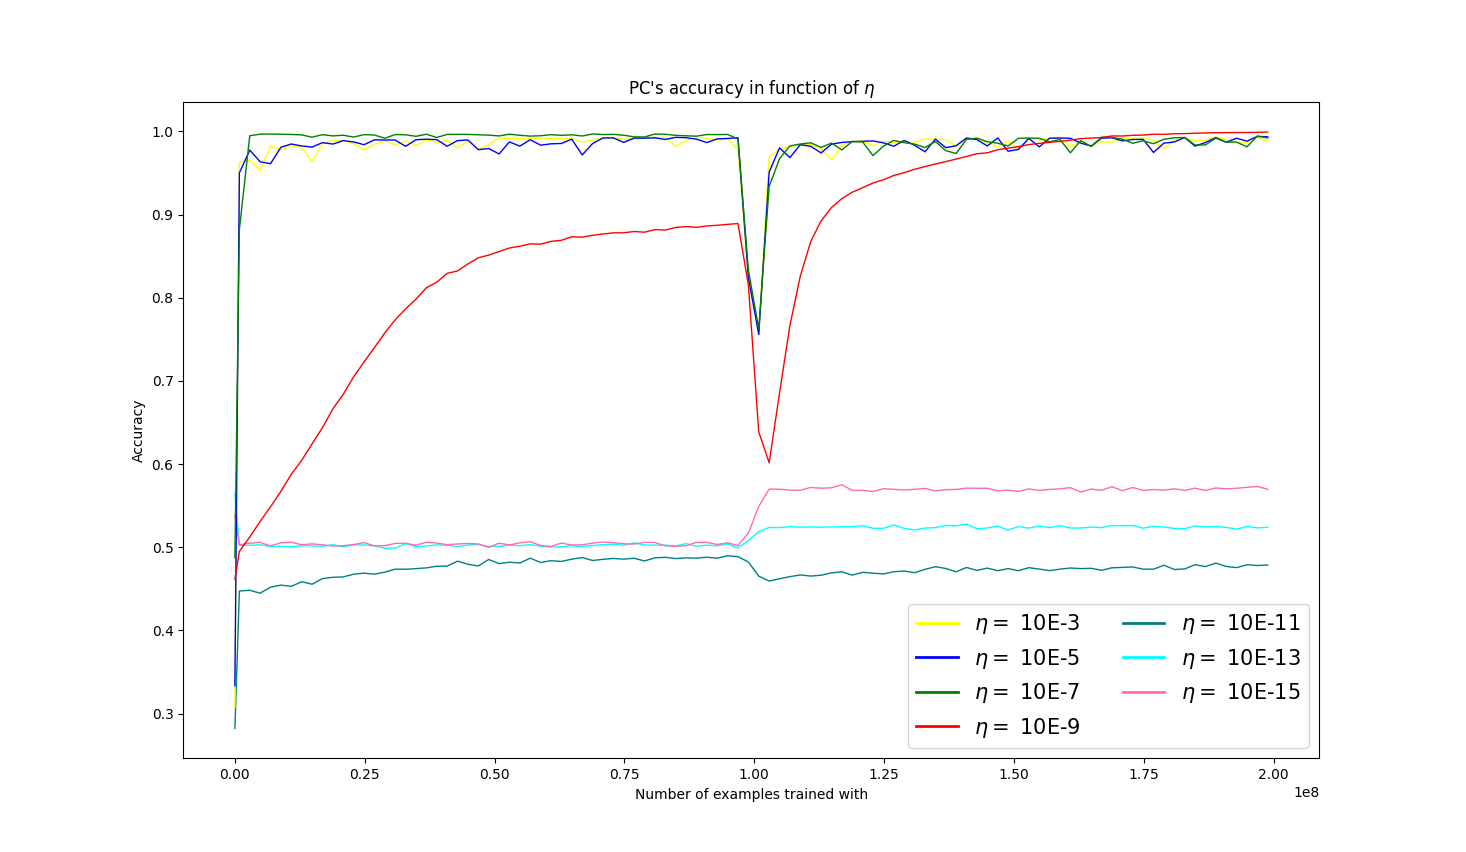
\includegraphics[width=1.6\linewidth, center]{./img/pc_etas.png}
	\caption{Effect of varying the learning rate $\eta$ (with weights initialised to non-zero values)}
	\label{fig:pc_etas}	
\end{figure}
\begin{figure}
	\centering
	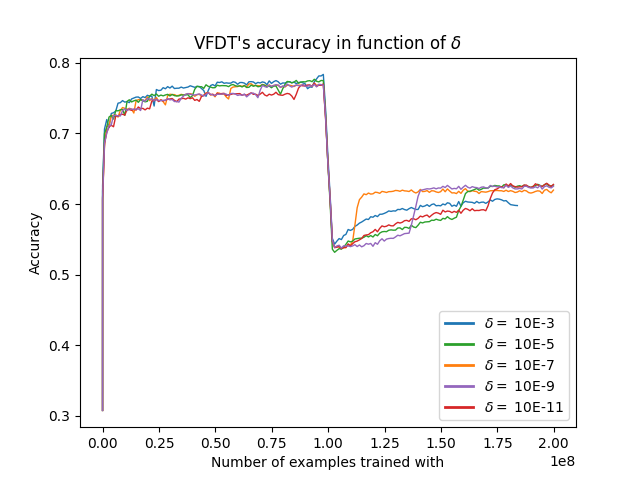
\includegraphics[width=.8\linewidth]{./img/vfdt_delta.png}
	\caption{Effect of varying $\delta$}
	\label{fig:vfdt_deltas}	
\end{figure}
\begin{figure}
	\centering
	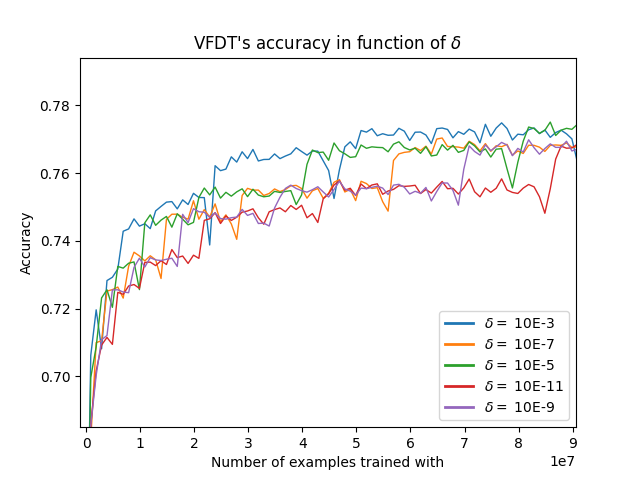
\includegraphics[width=.8\linewidth]{./img/vfdt_delta_zoom2.png}
	\caption{Enlarged view of figure \ref{fig:vfdt_deltas} (before concept drift)}
	\label{fig:vfdt_delta_zoom}	
\end{figure}
\begin{figure}
	\centering
	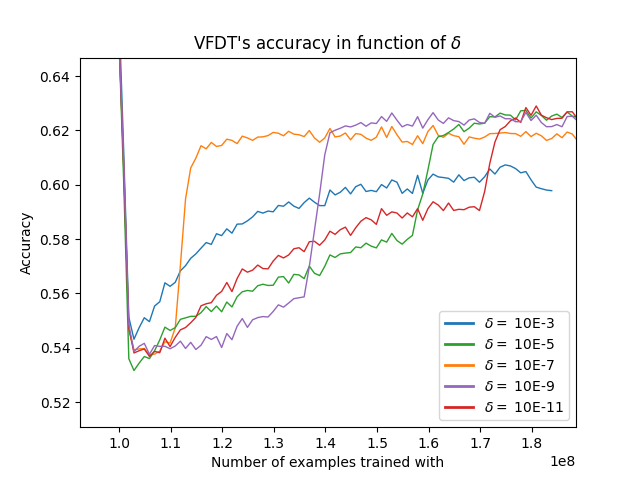
\includegraphics[width=.8\linewidth]{./img/vfdt_delta_zoom.png}
	\caption{Enlarged view of figure \ref{fig:vfdt_deltas} (after concept drift)}
	\label{fig:vfdt_delta_zoom2}	
\end{figure}
\begin{figure}
	\centering
	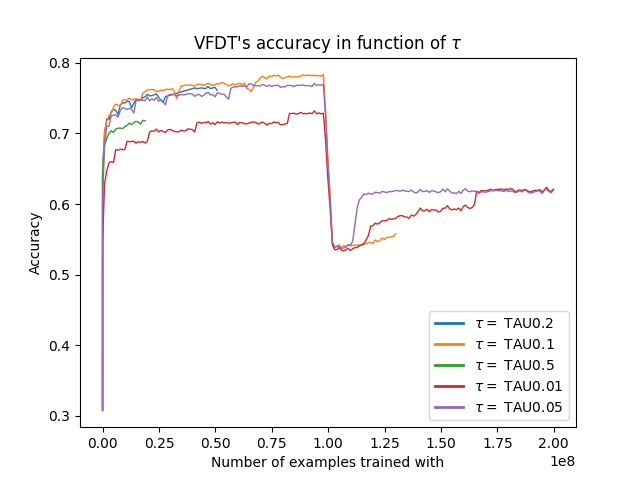
\includegraphics[width=.8\linewidth]{./img/vfdt_taus.png}
	\caption{Effect of varying $\tau$}
	\label{fig:vfdt_taus}	
\end{figure}
\begin{figure}
	\centering
	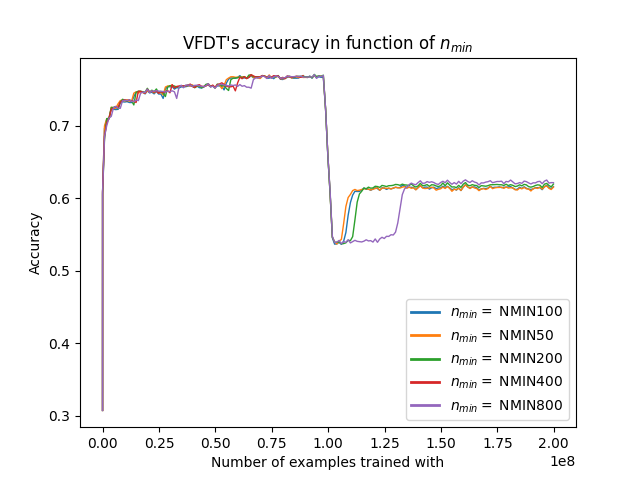
\includegraphics[width=.8\linewidth]{./img/vfdt_nmin.png}
	\caption{Effect of varying $n_{min}$}
	\label{fig:vfdt_nmins}	
\end{figure}
\begin{figure}
	\centering
	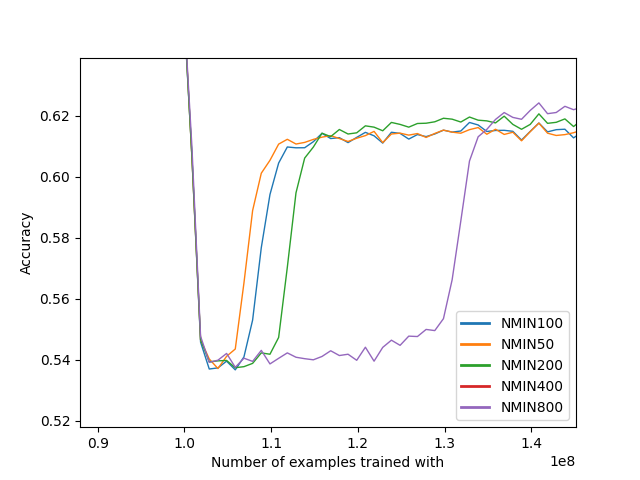
\includegraphics[width=.8\linewidth]{../code/experiments/vfdt/plots/vfdt_nmin_zoom.png}
	\caption{Enlarged view of figure \ref{fig:vfdt_nmins}}
	\label{fig:vfdt_nmins_zoom}	
\end{figure}



\end{document}
